\documentclass[conference]{IEEEtran}
\IEEEoverridecommandlockouts
% The preceding line is only needed to identify funding in the first footnote. If that is unneeded, please comment it out.
\usepackage{cite}
\usepackage{amsmath,amssymb,amsfonts}
\usepackage{algorithmic}
\usepackage{graphicx}
\usepackage{textcomp}
\usepackage[table,xcdraw]{xcolor}
\usepackage[utf8]{inputenc}
\usepackage[vietnamese]{babel}
\usepackage{float} 
\usepackage{multirow}
\usepackage{url}

\bibliographystyle{IEEEtran}

\def\BibTeX{{\rm B\kern-.05em{\sc i\kern-.025em b}\kern-.08em
    T\kern-.1667em\lower.7ex\hbox{E}\kern-.125emX}}
\begin{document}

\title{DỰ BÁO MỨC ĐỘ Ô NHIỄM KHÔNG KHÍ TẠI BA TỈNH MIỀN BẮC VIỆT NAM: PHƯƠNG PHÁP HỌC MÁY VÀ HỌC SÂU\\
{\footnotesize}
\thanks{Identify applicable funding agency here. If none, delete this.}
}

\author{\IEEEauthorblockN{1\textsuperscript{st} Cao Hoai Sang}
    \IEEEauthorblockA{\textit{Information System} \\
        \textit{name of organization (of Aff.)}\\
        Ho Chi Minh City, Viet Nam \\
        21522541@gm.uit.edu.vn}
    \and
    \IEEEauthorblockN{2\textsuperscript{nd} Nguyen Tran Gia Kiet}
    \IEEEauthorblockA{\textit{Information System} \\
        \textit{name of organization (of Aff.)}\\
        Ho Chi Minh City, Viet Nam \\
        21522258@gm.uit.edu.vn}
    \and
    \IEEEauthorblockN{3\textsuperscript{rd} Thi Thanh Cong}
    \IEEEauthorblockA{\textit{dept. name of organization (of Aff.)} \\
        \textit{name of organization (of Aff.)}\\
        City, Country \\
        email address or ORCID}
    \and
    \IEEEauthorblockN{4\textsuperscript{th} Nguyen Hoang Dang Khoa}
    \IEEEauthorblockA{\textit{dept. name of organization (of Aff.)} \\
        \textit{name of organization (of Aff.)}\\
        City, Country \\
        email address or ORCID}
    \and
    \IEEEauthorblockN{5\textsuperscript{th} Cu Ngoc Hoang}
    \IEEEauthorblockA{\textit{dept. name of organization (of Aff.)} \\
        \textit{name of organization (of Aff.)}\\
        City, Country \\
        email address or ORCID}
    \and
    \IEEEauthorblockN{6\textsuperscript{th} Given Name Surname}
    \IEEEauthorblockA{\textit{dept. name of organization (of Aff.)} \\
        \textit{name of organization (of Aff.)}\\
        City, Country \\
        email address or ORCID}
}

\maketitle

\begin{abstract}
    Mục tiêu chính của nghiên cứu này là dự đoán chất lượng không khí của ba tỉnh được chỉ định (Bắc Ninh, Hà Nội và Quảng Ninh) ở khu vực phía Bắc Việt Nam bằng cách kết hợp các thuật toán học máy và học sâu. Các mô hình bao gồm Gauss Newton Method Non-Linear, Residual Convolutional Neural Networks (ResCNN), Neural Hierarchical Interpolation for Time Series Forecasting (N-HiTS), Dynamic Linear Model (DLM), Simple Exponential Smoothing (SES), Linear Regression (LR), Autoregressive Integrated Moving Average (ARIMA), Recurrent Neural Network (RNN), Gated Recurrent Unit (GRU), Long Short Term Memory (LSTM). Hiệu quả của tất cả các mô hình được đề cập trên được đo lường bằng Mean Absolute Percentage Error (MAPE), Root Mean Squared Error, nhằm đạt được độ chính xác tối đa trong dự báo chuỗi thời gian chất lượng không khí chính xác.
\end{abstract}

\begin{IEEEkeywords}
    Nonlinear regression, Gauss-Newton, generalized least squares, iteratively reweighted least
    squares
\end{IEEEkeywords}

\section{Giới Thiệu}
Với sự gia tăng dân số nhanh chóng ở Việt Nam cùng với sự công nghiệp hóa ngày càng mạnh mẽ ở các khu vực trọng yếu, vấn đề chất lượng không khí nhanh chóng trở thành mối quan tâm chính, đặc biệt là ở các tỉnh đông dân cư ở khu vực phía Bắc Việt Nam. Sự suy giảm chất lượng không khí không chỉ gây ra những rủi ro lớn đối với sức khỏe của cư dân mà còn đe dọa sự cân bằng sinh thái mong manh của khu vực. Trong bối cảnh này, việc dự đoán chính xác và kịp thời các mức độ chất lượng không khí là rất cần thiết cho các chiến lược giảm thiểu hiệu quả và can thiệp y tế công cộng. Nghiên cứu của nhóm chúng tôi sử dụng sự kết hợp của các mô hình học máy và học sâu để dự đoán chất lượng không khí, bằng cách tận dụng sức mạnh của các thuật toán phức tạp như Gauss Newton Method Non-Linear, Resilient Convolutional Neural Networks (ResCNN), Neural Hierarchical Interpolation for Time Series Forecasting (N-HiTS), Dynamic Linear Model (DLM), Simple Exponential Smoothing (SES), Linear Regression (LR), Autoregressive Integrated Moving Average (ARIMA), Recurrent Neural Network (RNN), Gated Recurrent Unit (GRU), và Long Short Term Memory (LSTM).

Việc bao gồm một tập hợp đa dạng các mô hình cho phép chúng tôi khám phá các khía cạnh khác nhau của dữ liệu và so sánh hiệu suất của các phương pháp khác nhau. Chẳng hạn, các mô hình thống kê truyền thống như SES, LR, và ARIMA cung cấp tính giải thích và sự đơn giản, làm cho chúng trở thành các mô hình cơ sở có giá trị để so sánh. Mặt khác, các kiến trúc học sâu như RNN, GRU, và LSTM xuất sắc trong việc nắm bắt các phụ thuộc phi tuyến tính và phụ thuộc thời gian dài hạn, những đặc điểm thường có trong dữ liệu chuỗi thời gian chất lượng không khí. Ngoài ra, các phương pháp sáng tạo như ResCNN và N-HiTS mang lại những lợi thế độc đáo trong việc xử lý các cấu trúc không gian và thứ bậc trong dữ liệu, nâng cao độ chính xác của các dự đoán.

\section{Nghiên cứu liên quan}

\subsection{Gauss-Newton nonlinear method}

Vào năm 2015, ứng dụng dự báo phục hồi sau xuất viện của Phạm Thị Hương được
sử dụng trong luận văn thạc sĩ khoa học [1]. Sử dụng phương pháp Gauss-Newton
phi tuyến để ước lượng giá trị nhỏ nhất của bình phương sai số. \cite{b1}

\subsection{ResCNN}
Phân loại ECG bằng bộ Ensemble của Residual CNNs với Cơ chế Chú ý.

Trong phân loại ECG, sử dụng ResNet kết hợp với cơ chế chú ý đa đầu đã chứng minh hiệu quả. Giải pháp của Đội ISIBrno-AIMT trong Cuộc thi PhysioNet 2021 đã thể hiện sự vượt trội bằng việc phân loại ECG thành 26 nhóm khác nhau. Phương pháp này tích hợp các hàm mất mát và tối ưu hóa tiến hóa, mang lại đóng góp quan trọng cho lĩnh vực này. \cite{b4}

\section{Tài nguyên}
\subsection{Bộ dữ liệu}
Dự báo chất lượng không khí là rất quan trọng để giảm thiểu các tác động tiêu cực của ô nhiễm lên sức khỏe con người và môi trường. Phân tích chuỗi thời gian nổi lên như một công cụ mạnh mẽ trong lĩnh vực này, cho phép dự đoán các mức độ chất lượng không khí trong tương lai dựa trên dữ liệu lịch sử.

Do các vấn đề phổ biến liên quan đến bụi mịn ở khu vực phía Bắc, nhóm đã chọn một bộ dữ liệu chi tiết về chất lượng không khí của ba thành phố lớn ở miền Bắc Việt Nam: Bắc Ninh, Hà Nội và Quảng Ninh.

Bộ dữ liệu chủ yếu kéo dài từ năm 2021 đến năm hiện tại, 2024, bao gồm 6 cột tương ứng với các thành phần khác nhau trong không khí và chất lượng không khí được đánh giá thông qua Chỉ số Chất lượng Không khí (AQI): nồng độ PM2.5, nồng độ PM10, nồng độ O3, nồng độ NO2, nồng độ SO2 và nồng độ CO.
\subsection{Thống kế mô tả}

\begin{table}[H]
    \centering
    \caption{HaNoi, BacNinh, QuangNinh’s Descriptive Statistics}
    \begin{tabular}{|>{\columncolor{red!20}}c|c|c|c|}
        \hline
        \rowcolor{red!20} & HaNoi  & BacNinh & QuangNinh \\ \hline
        Count             & 2779   & 1190    & 929       \\ \hline
        Mean              & 75.283 & 86.87   & 32.117    \\ \hline
        Std               & 42.635 & 43.484  & 25.576    \\ \hline
        Min               & 11     & 10.0    & 5.0       \\ \hline
        25\%              & 42.0   & 59.0    & 19.0      \\ \hline
        50\%              & 66.0   & 72.0    & 25.0      \\ \hline
        75\%              & 101.0  & 111.0   & 38.0      \\ \hline
        Max               & 498    & 275.0   & 500.0     \\ \hline
    \end{tabular}
\end{table}

\begin{figure}[H]
    \centering
    \begin{minipage}{0.23\textwidth}
        \centering
        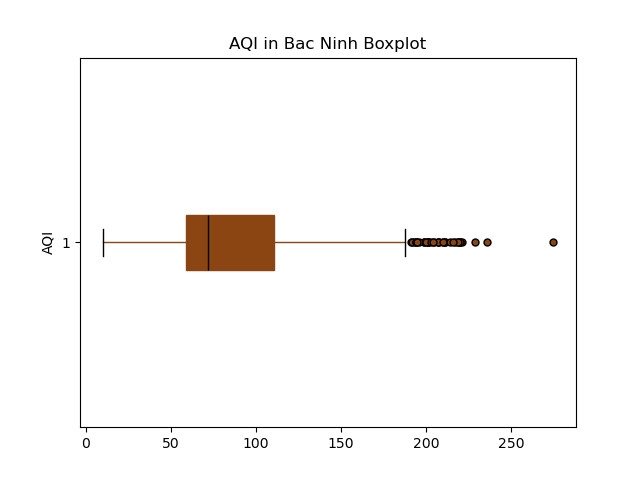
\includegraphics[width=1\textwidth]{bibliography/figure/bn_box.jpg}
        \caption{BacNinh AQI's boxplot}
        \label{fig:1}
    \end{minipage}
    \hfill
    \begin{minipage}{0.23\textwidth}
        \centering
        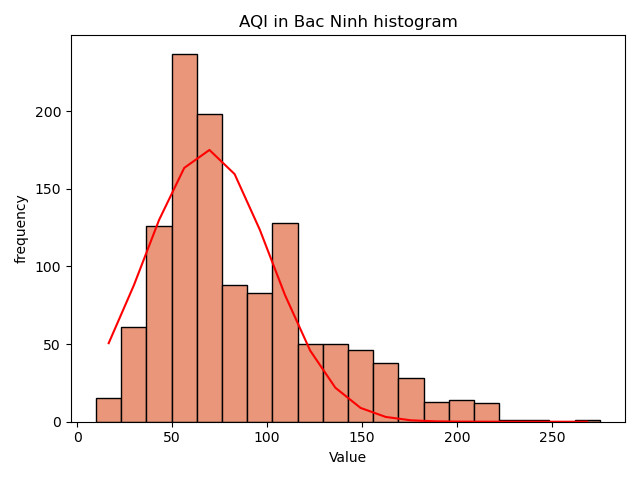
\includegraphics[width=1\textwidth]{bibliography/figure/bn_his.jpg}
        \caption{BacNinh AQI's hostogram}
        \label{fig:2}
    \end{minipage}
\end{figure}

\begin{figure}[H]
    \centering
    \begin{minipage}{0.23\textwidth}
        \centering
        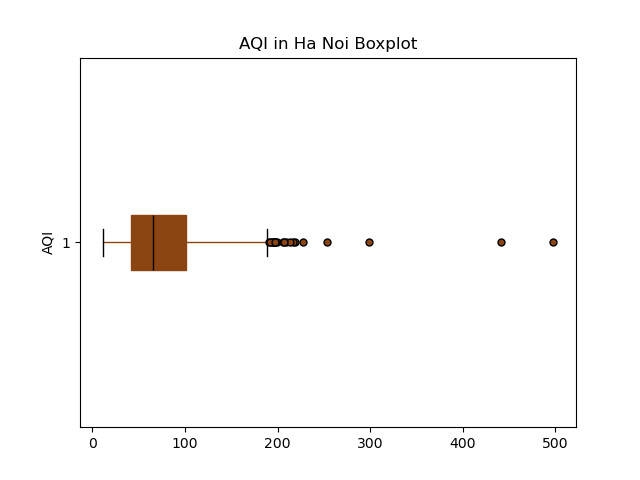
\includegraphics[width=1\textwidth]{bibliography/figure/hn_box.jpg}
        \caption{HaNoi AQI's boxplot}
        \label{fig:1}
    \end{minipage}
    \hfill
    \begin{minipage}{0.23\textwidth}
        \centering
        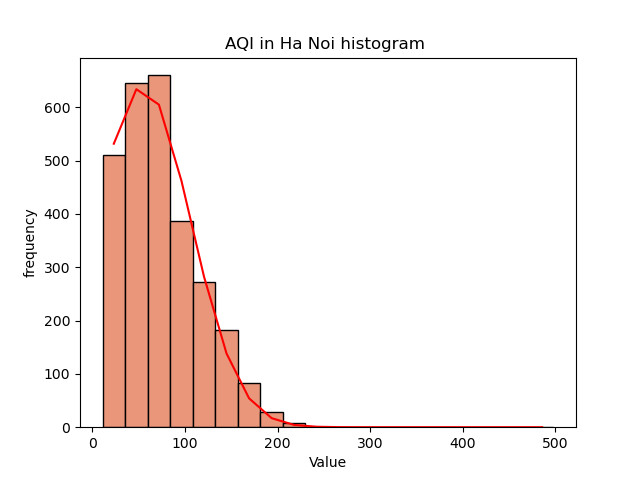
\includegraphics[width=1\textwidth]{bibliography/figure/hn_his.jpg}
        \caption{HaNoi AQI's hostogram}
        \label{fig:2}
    \end{minipage}
\end{figure}

\begin{figure}[H]
    \centering
    \begin{minipage}{0.23\textwidth}
        \centering
        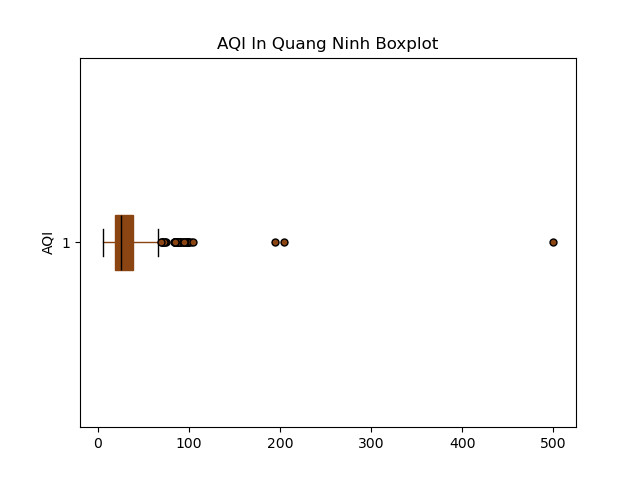
\includegraphics[width=1\textwidth]{bibliography/figure/qn_box.jpg}
        \caption{QuangNinh AQI's boxplot}
        \label{fig:1}
    \end{minipage}
    \hfill
    \begin{minipage}{0.23\textwidth}
        \centering
        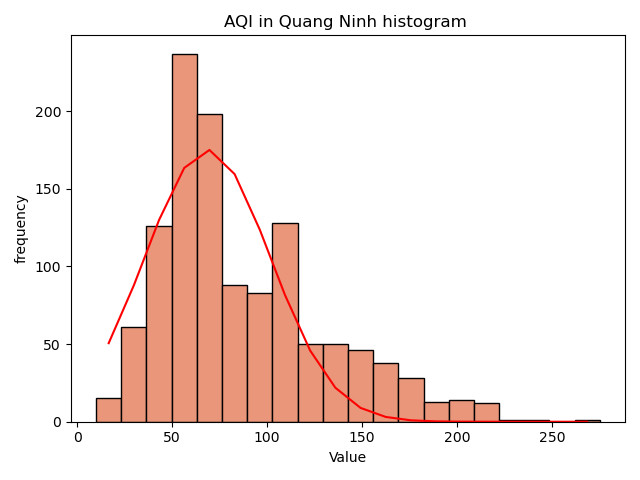
\includegraphics[width=1\textwidth]{bibliography/figure/qn_his.jpg}
        \caption{QuangNinh AQI's hostogram}
        \label{fig:2}
    \end{minipage}
\end{figure}

\section{Phương pháp luận}
\subsection{Gauss newton method nonlinear}
\subsubsection{Least Squares}
Khoảng cách giữa một đường cong được khớp và một quan sát được gọi là sai số dư, hoặc lỗi.

\begin{center}
    $Residuals = y_i - \widehat{y}_i$
\end{center}

Tổng của các sai số bình phương được tính bằng phương trình sau:

\begin{center}
    $SSE = \sum_{i=1}^{n}(y_i - \widehat{y}_i)^2$
\end{center}

Trong đó: \\
\indent\textbullet\ \(y_i\) là các giá trị quan sát được\\
\indent\textbullet\ \(\widehat{y}_i\) là các giá trị khớp\\

\subsubsection{Phương pháp Newton}
Với hàm \( y = y_0 e^{-kt} \), chúng ta tìm giá trị nhỏ nhất của SSE. Chúng ta tìm giá trị \(k\) bằng phương pháp Newton.

\begin{center}
    $SSE = \sum_{i}^{n}(y_i - y_0 e^{-kt_i})^2$
\end{center}

\begin{center}
    \(k_{\text{new}} = k_{\text{old}} - \frac{f'(k_{\text{old}})}{f''(k_{\text{old}})}\)
\end{center}

Hoặc chúng ta có thể giải thích bằng ma trận Hessian như sau:

\begin{center}
    \[
        \begin{pmatrix}
            k_{\text{new}} \\ y_{0,\text{new}}
        \end{pmatrix} =
        \begin{pmatrix}
            k_{\text{old}} \\ y_{0,\text{old}}
        \end{pmatrix} - H^{-1}G
    \]
\end{center}

Trong đó: \\
\indent\textbullet\ \(H = \begin{bmatrix}
    \frac{\partial^2 f}{\partial k^2}            & \frac{\partial^2 f}{\partial k \partial y_0} \\
    \frac{\partial^2 f}{\partial y_0 \partial k} & \frac{\partial^2 f}{\partial y_0^2}
\end{bmatrix}\)\\
\indent\textbullet\ \(G = \begin{bmatrix}
    \frac{\partial f}{\partial k} \\ \frac{\partial f}{\partial y_0}
\end{bmatrix}\)\\

Vấn đề với phương pháp Newton trong hồi quy phi tuyến là việc tính toán ma trận Hessian và nghịch đảo của nó gặp khó khăn. Để giải quyết vấn đề này, phương pháp Gauss-Newton thay thế bằng cách xấp xỉ ma trận Hessian.

Chúng ta có thể viết lại SSE như sau:
\begin{center}
    $SSE = \sum_{i}^{n}r_i^2 = r^T r$
\end{center}

Trong đó: \\
\indent\textbullet\ \(r\) là một vector chứa các sai số dư \\

\subsubsection{Phương pháp Gauss-Newton}
Chúng ta lấy đạo hàm của SSE theo các tham số trong mô hình bằng quy tắc chuỗi, chúng ta có được phương trình sau:
\begin{center}
    \(
    \frac{\partial SSE}{\partial \beta_j} = 2\sum_{i}^{n} r_i \frac{\partial r_i}{\partial \beta_j}
    \)
\end{center}

Sau đó, bỏ số hai vì nó sẽ không ảnh hưởng đến việc ước tính các tham số. Tương ứng với ma trận Jacobian.

\begin{center}
    \(
    J_r = \begin{bmatrix}
        \frac{\partial r_1}{\partial \beta_1} & \frac{\partial r_1}{\partial \beta_2} \\
        \frac{\partial r_2}{\partial \beta_1} & \frac{\partial r_2}{\partial \beta_2} \\
        \vdots                                & \vdots                                \\
        \frac{\partial r_n}{\partial \beta_1} & \frac{\partial r_n}{\partial \beta_2}
    \end{bmatrix}
    \)
\end{center}

Với phương trình sau cho tổng các sai số bình phương (SSE):
\[
    SSE = \sum_{i=1}^{n} (y_i - y_0 e^{-kt_i})^2
\]
Chúng ta có:
\begin{center}
    \(
    \frac{\partial^2 {SSE}}{\partial \beta_j \partial \beta_k} = \sum_{i}^{n} \left( \frac{\partial r_i}{\partial \beta_j} \frac{\partial r_i}{\partial \beta_k} + r_i \frac{\partial^2 r_i}{\partial \beta_j \partial \beta_k} \right)
    \)
\end{center}

Sự khác biệt chính giữa phương pháp Newton và Gauss-Newton là phương pháp Gauss-Newton bỏ qua \(r_i \frac{\partial^2 r_i}{\partial \beta_j \partial \beta_k}\).
Do đó, đạo hàm bậc hai được xấp xỉ bằng hàm sau:
\begin{center}
    \(
    \frac{\partial^2 {SSE}}{\partial \beta_j \partial \beta_k} \approx \sum_{i}^{n} \left( \frac{\partial r_i}{\partial \beta_j} \frac{\partial r_i}{\partial \beta_k} \right) = J^T_r J_r
    \)
\end{center}

Sử dụng quy tắc cập nhật sau trong phương pháp Newton. Đối với Gauss-Newton, đơn giản chỉ cần cắm vào xấp xỉ cho ma trận Hessian và gradient.

\begin{center}
    \[
        \begin{pmatrix}
            k_{\text{new}} \\ y_{0,\text{new}}
        \end{pmatrix} =
        \begin{pmatrix}
            k_{\text{old}} \\ y_{0,\text{old}}
        \end{pmatrix} - (J^T_r J_r)^{-1} J^T_r r
    \]
\end{center}

Với \(\beta\) là một vector cột với các tham số được ước tính. Đối với ví dụ đơn giản chỉ ước tính hai tham số, phương trình trông như sau:

\begin{center}
    \[
        \beta_{\text{new}} = \beta_{\text{old}} - (J^T_r J_r)^{-1} J^T_r r(\beta_{\text{old}})
    \]
    \[
        \begin{pmatrix}
            k_{\text{new}} \\ y_{0,\text{new}}
        \end{pmatrix} =
        \begin{pmatrix}
            k_{\text{old}} \\ y_{0,\text{old}}
        \end{pmatrix} - (J^T_r J_r)^{-1} J^T_r r \begin{pmatrix}
            k_{\text{old}} \\ y_{0,\text{old}}
        \end{pmatrix}
    \]
\end{center}
\vspace{3mm}
\subsection{AUTOREGRESSIVE INTEGRATED MOVING AVERAGE (ARIMA)}

ARIMA là viết tắt của "Autoregressive Integrated Moving Average". Mô hình ARIMA thường được sử dụng để dự báo dữ liệu chuỗi thời gian đơn biến. Mô hình ARIMA có thể xử lý một chuỗi thời gian nếu chuỗi đó là dừng và không có dữ liệu bị thiếu. Phương pháp này được sử dụng trong nhiều nghiên cứu để dự báo. 

ARIMA là sự kết hợp của 3 thành phần, Auto-Regressive – AR, Integrated – I và Moving Average – MA tương ứng với các tham số p, d và q đại diện cho ba thành phần chính của mô hình, trong đó:
\\
\indent\textbullet\ \(p-AR(p)\): Tham số p đại diện cho số lượng các quá trình tự hồi quy trong thành phần tự hồi quy (AutoRegressive) của mô hình ARIMA. Nó chỉ ra số lượng ngày quá khứ của chuỗi dữ liệu mà được sử dụng để dự đoán giá trị hiện tại. Mỗi giá trị quá khứ được sử dụng là một hệ số trong mô hình tự hồi quy. Giá trị của p phụ thuộc vào sự phụ thuộc tạm thời trong chuỗi dữ liệu và có thể được xác định bằng cách sử dụng các phương pháp như đồ thị tự tương quan (ACF - AutoCorrelation Function) hoặc hàm tương quan một lệnh (PACF - Partial AutoCorrelation Function). Phương trình tự hồi quy AR được tổng quát như sau:\\
\[
Y_t = c + \varphi_1 Y_{t-1} + \varphi_2 Y_{t-2} + \ldots + \varphi_p Y_{t-p} + \epsilon_t
\]
Trong đó: \\
\indent -- \(Y_t\) đại diện cho giá trị dữ liệu tại thời điểm t\\
\indent -- \(c\) là hằng số chặn\\
\indent -- \(\varphi\) là hệ số AutoRegressive(AR)\\
\indent -- \(\epsilon_t\) là sai số ngẫu nhiên \\
\indent -- \(p\) là số bậc \\

\indent\textbullet\ \(q-MA(q)\): Tham số q đại diện cho số lượng các thành phần trung bình động (Moving Average) trong mô hình ARIMA. Nó chỉ ra số lượng giá trị trung bình động được sử dụng để dự đoán giá trị hiện tại.\\
\[
Y_t = c + \theta_1 \epsilon_{t-1} + \theta_2 \epsilon_{t-2} + \ldots + \theta_p \epsilon_{t-p} + \epsilon_t
\]

Trong đó: \\
\indent -- \(Y_t\) đại diện cho giá trị dữ liệu tại thời điểm t\\
\indent -- \(c\) là hằng số chặn\\
\indent -- \(\theta\) là hệ số Moving Average(MA)\\
\indent -- \(\epsilon_t\) là hệ số tương quan\\
\indent -- \(p\) là số bậc \\

\indent\textbullet\  \(d-I(d)\): Tham số d đại diện cho số lần lấy đạo hàm-sai phân (differencing) trên chuỗi dữ liệu ban đầu để loại bỏ xu hướng (trend) và/hoặc thành phần mùa vụ (seasonality) hay chuyển đổi dữ liệu thành chuỗi dừng. chuỗi dừng là chuỗi có trung bình, phương sai và tự tương quan không đổi theo thời gian. Một chuỗi thời gian được coi là chuỗi dừng nếu nó có trung bình không đổi, phương sai không đổi và tự tương quan không đổi. Chuỗi dừng là Công thức tính sai phân tại thời điểm t như sau
\[
    \Delta y_t = y_t - y_{t-1}
\]

Sau khi kết hợp tất cả, ta có ARIMA(p, d, q) được biểu diễn như sau:
\[
    \Delta y_t = c + \varphi_1 \Delta y_{t-1} + \ldots + \varphi_p \Delta y_{t-p} + \varepsilon_t + \theta_1 \varepsilon_{t-1} + \theta_1 \varepsilon_{t-1} + \ldots + \theta_q \varepsilon_{t-q}
\]

Trong đó: \\
\indent -- \(Y_t\) đại diện cho giá trị dữ liệu tại thời điểm t\\
\indent -- \(c\) là hằng số chặn\\
\indent -- \(\theta\) là hệ số Moving Average(MA)\\
\indent -- \(\epsilon_t\) là hệ số tương quan\\
\indent -- \(\varphi\) là hệ số AutoRegressive(AR)\\

\subsection{LSMT ResCNN}
\subsubsection{Tổng quan}
Mô hình LSTM ResCNN là một mô hình dự đoán chuỗi thời gian, là sự kết hợp giữa LSTM và CNN 1D sử dụng kết nối bỏ qua.
\subsubsection{1D-CNN}
CNN phổ biến nhất được biết đến là CNN 2D, chủ yếu được sử dụng trong xử lý ảnh. Ngoài ra còn có CNN 1D được sử dụng trong xử lý ngôn ngữ tự nhiên và phân tích chuỗi thời gian, nó trích xuất các đặc trưng bằng cách di chuyển kernel dọc theo trục thời gian. Lớp CNN 1D đóng góp vào việc trích xuất các đặc trưng vốn có trong dữ liệu, và số lượng bộ lọc xác định số lượng đặc trưng cần được học, phù hợp với kích thước của không gian đầu ra.
\subsubsection{LSTM-ResCNN được đề xuất với cách tiếp cận dựa trên độ dốc}
\paragraph{Giới thiệu mô hình}
Trong bài báo này, chúng tôi đề xuất một mô hình LSTM-resCNN, đó là một LSTM-CNN với một kết nối dư thêm trên các lớp CNN 1D. Lý do chúng tôi chọn thứ tự LSTM-CNN thay vì CNN-LSTM là để đặt lớp tích chập mà Grad-CAM có thể được áp dụng ở phần sau để biểu diễn các đặc trưng phức tạp hơn. Chúng tôi đã bao gồm một kết nối dư để tránh mất thông tin quan trọng trong quá trình áp dụng ba lớp tích chập 1D liên tục. Ngoài ra, các mạng dư đã chứng minh rằng chúng có thể được coi như một sự kết hợp của nhiều đường đi khác nhau với độ dài khác nhau, và các đường đi này thể hiện hành vi giống như một tổ hợp.
\paragraph{Thiết kế mô hình}
Mô hình LSTM-resCNN được đề xuất được mô tả trong Bảng 2. Mỗi khối CNN bao gồm ba lớp CNN 1D với kích thước bộ lọc là 64 mỗi lớp và kích thước kernel là 3, 2 và 1. Kích thước bộ lọc 64 được chọn từ giữa 32, 64 và 128 dựa trên tìm kiếm siêu tham số. Một kết nối dư được thêm vào mỗi khối CNN. Sau khi áp dụng hai khối CNN, một lớp flatten được áp dụng để chuyển đổi các đặc trưng thành các vector một chiều. Tiếp theo, một lớp dropout được sử dụng để ngăn chặn việc quá mức hóa. Cuối cùng, kết quả được chuyển đến lớp dense. Kích thước của bộ lọc là 1 và 24 cho các mô hình dự đoán một bước và nhiều bước tương ứng.
\begin{center}
    \begin{table}[h!]
        \centering
        \begin{tabular}{|c|c|c|p{2cm}|}
            \hline
            \textbf{Models}                       & \multicolumn{2}{c|}{\textbf{Layer}}   & \textbf{Parameters}                                                                                      \\ \hline
            \multirow{9}{*}{\textbf{LSTM-resCNN}} & \multicolumn{2}{c|}{LSTM}             & \makebox[3cm]{Filter = 64}                                                                               \\ \cline{2-4}
                                                  & \multirow{4}{*}{CNN-Block $\times$ 2} & 1D-CNN                     & \begin{tabular}{@{}l@{}}Filter=64,\\ kernel-size=3,\\ stride=1\end{tabular} \\ \cline{3-4}
                                                  &                                       & 1D-CNN                     & \begin{tabular}{@{}l@{}}Filter=64,\\ kernel-size=2,\\ stride=1\end{tabular} \\ \cline{3-4}
                                                  &                                       & 1D-CNN                     & \begin{tabular}{@{}l@{}}Filter=64,\\ kernel-size=1,\\ stride=1\end{tabular} \\ \cline{3-4}
                                                  &                                       & Add                        &                                                                             \\ \cline{2-4}
                                                  & \multicolumn{2}{c|}{Flatten}          &                                                                                                          \\ \cline{2-4}
                                                  & \multicolumn{2}{c|}{Dropout}          & \makebox[3cm]{p = 0.5}                                                                                   \\ \cline{2-4}
                                                  & \multicolumn{2}{c|}{Dense}            &                                                                                                          \\ \hline
        \end{tabular}
        \caption{cấu trúc model LSTM ResCNN}
        \label{tab:lstm-rescnn}
    \end{table}
\end{center}


\subsection{Gated Recurrent Unit (GRU)}
\subsubsection{Đơn vị tuần hoàn trong mạng nơ-ron}
Trước khi chúng ta đi vào chi tiết về GRU, hãy xem xét một đơn vị tuần hoàn thông thường trong mạng nơ-ron. Đơn vị này được sử dụng để xử lý dữ liệu tuần tự, chẳng hạn như chuỗi văn bản, âm thanh hoặc dữ liệu thời gian.

Mỗi đơn vị tuần hoàn có một trạng thái ẩn (hidden state) và nhận đầu vào từ bước thời gian trước đó. Nó sử dụng thông tin từ trạng thái ẩn và đầu vào hiện tại để tính toán trạng thái ẩn mới.

\subsubsection{GRU là gì?}
GRU là một biến thể của đơn vị tuần hoàn, được thiết kế để giải quyết một số vấn đề của kiến trúc LSTM (Long Short-Term Memory).

Sự khác biệt chính giữa GRU và LSTM nằm ở cách xử lý trạng thái ẩn và ô nhớ:

\begin{itemize}
    \item \textbf{LSTM}: Sử dụng ba cổng (input gate, output gate và forget gate) để duy trì trạng thái của ô nhớ riêng biệt.
    \item \textbf{GRU}: Không có ô nhớ riêng biệt, thay vào đó, nó sử dụng một “vector kích hoạt ứng viên” và hai cổng (reset gate và update gate).
\end{itemize}

\begin{itemize}
    \item \textbf{Cổng đặt lại (reset gate)}: Quyết định bao nhiêu trạng thái ẩn trước đó cần quên.
    \item \textbf{Cổng cập nhật (update gate)}: Quyết định bao nhiêu của vector kích hoạt ứng viên cần tích hợp vào trạng thái ẩn mới.
\end{itemize}

\subsubsection{Cổng xóa và cổng cập nhật}
Đầu tiên ta giới thiệu cổng xóa và cổng cập nhật. Ta thiết kế chúng thành các vector có các phần tử trong khoảng  (0,1)
để có thể biểu diễn các tổ hợp lồi. Chẳng hạn, một biến xóa cho phép kiểm soát bao nhiêu phần của trạng thái trước đây được giữ lại. Tương tự, một biến cập nhật cho phép kiểm soát bao nhiêu phần của trạng thái mới sẽ giống trạng thái cũ.


\begin{figure}[H]
    \centering
    \begin{minipage}{0.23\textwidth}
        \centering
        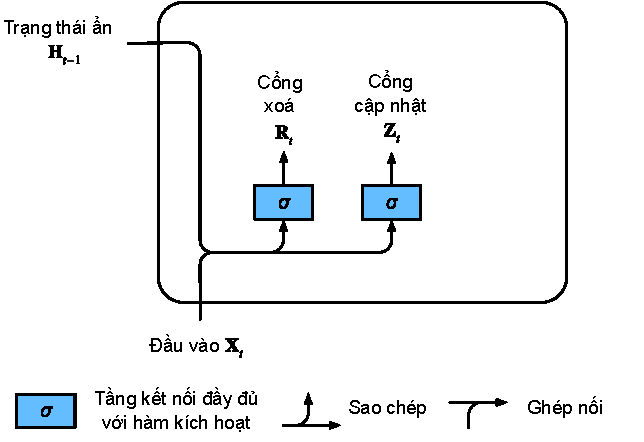
\includegraphics[width=1\textwidth]{bibliography/figure/GRU/gru_1.pdf}
        \caption{Cổng xóa và cổng cập nhật trong GRU}
        \label{fig:gru_del_up}
    \end{minipage}

\end{figure}

Ta bắt đầu bằng việc thiết kế các cổng tạo ra các biến này. Hình \ref{fig:gru_del_up}
minh họa các đầu vào cho cả cổng xóa và cổng cập nhật trong GRU, với đầu vào ở bước thời gian hiện tại  \(\mathbf{X}_t \)
và trạng thái ẩn ở bước thời gian trước đó  \(\mathbf{H}_{t-1} \). Đầu ra được tạo bởi một tầng kết nối đầy đủ với hàm kích hoạt sigmoid.

Tại bước thời gian $t$, với đầu vào minibatch là $\mathbf{X}_t \in \mathbb{R}^{n \times d}$ (số lượng mẫu: $n$, số lượng đầu vào: $d$) và trạng thái ẩn ở bước thời gian gần nhất là $\mathbf{H}_{t-1} \in \mathbb{R}^{n \times h}$ (số lượng trạng thái ẩn: $h$), cổng xóa $\mathbf{R}_t \in \mathbb{R}^{n \times h}$ và cổng cập nhật $\mathbf{Z}_t \in \mathbb{R}^{n \times h}$ được tính như sau:

\begin{equation*}
    \mathbf{R}_t = \sigma(\mathbf{X}_t \mathbf{W}_{xr} + \mathbf{H}_{t-1} \mathbf{W}_{hr} + \mathbf{b}_r)
\end{equation*}
\begin{equation*}
    \mathbf{Z}_t = \sigma(\mathbf{X}_t \mathbf{W}_{xz} + \mathbf{H}_{t-1} \mathbf{W}_{hz} + \mathbf{b}_z).
\end{equation*}

Ở đây, $\mathbf{W}_{xr}, \mathbf{W}_{xz} \in \mathbb{R}^{d \times h}$ và $\mathbf{W}_{hr}, \mathbf{W}_{hz} \in \mathbb{R}^{h \times h}$ là các tham số trọng số và $\mathbf{b}_r, \mathbf{b}_z \in \mathbb{R}^{1 \times h}$ là các hệ số điều chỉnh. Ta sẽ sử dụng hàm sigmoid để biến đổi các giá trị đầu vào nằm trong khoảng $(0, 1)$.

\subsubsection{Hoạt động của cổng xóa}
Trong RNN thông thường, ta cập nhật trọng thái cổng xóa theo công thức
\[
    \mathbf{H}_t = \tanh(\mathbf{X}_t \mathbf{W}_{xh} + \mathbf{H}_{t-1} \mathbf{W}_{hh} + \mathbf{b}_h).
\]

Hình \ref{fig:gru_del} minh họa luồng tính toán sau khi áp dụng cổng xóa. Ký hiệu \(\bigodot\) biểu thị phép nhân theo từng phần tử giữa các tensor.

\begin{figure}[H]
    \centering
    \begin{minipage}{0.23\textwidth}
        \centering
        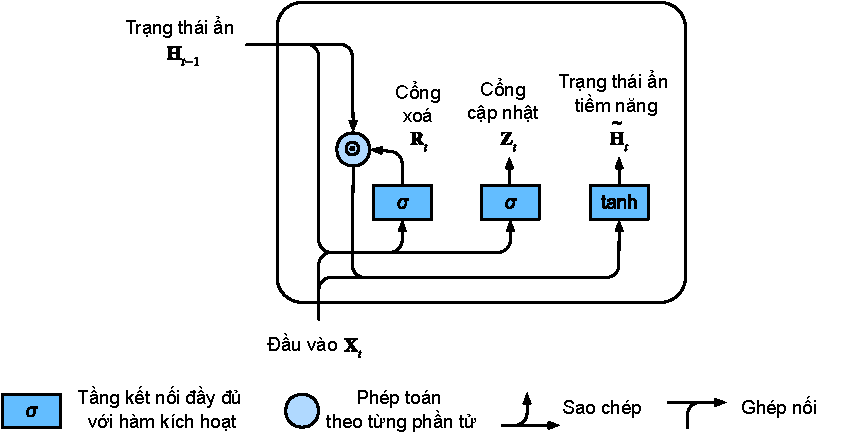
\includegraphics[width=1\textwidth]{bibliography/figure/GRU/gru_2.pdf}
        \caption{Tính toán trạng thái tiềm năng trong một GRU. Phép nhân được thực hiện theo phần tử}
        \label{fig:gru_del}
    \end{minipage}

\end{figure}

\begin{equation*}
    \tilde{\mathbf{H}}_t = \tanh (\mathbf{X}_t \mathbf{W}_{xh} + (\mathbf{R}_t \odot \mathbf{H}_{t-1}) \mathbf{W}_{hh} + \mathbf{b}_h).
\end{equation*}

\subsubsection{Hoạt động của cổng cập nhật}
Cổng này xác định mức độ giống nhau giữa tráng thái mới \(\mathbf{H}_t \) và trạng thái cũ \(\mathbf{H}_{t-1}\) cũng như mức độ trạng thái tiềm năng \(\widetilde{\mathbf{H}}_t\) được sử dụng. Biến cổng (gating variable) \(\mathbf{Z}_t\) được sử dụng cho mục đích này bằng cách áp dụng tổ hợp lồi giữa trạng thái cũ và trạng thái tiềm năng. Ta có phương
trình cập nhật cuối cho GRU.

\begin{equation*}
    \mathbf{H}_t = \mathbf{Z}_t \circ \mathbf{H}_{t-1} + (1 - \mathbf{Z}_t) \circ \tilde{\mathbf{H}}_t.
\end{equation*}

\begin{figure}[H]
    \centering
    \begin{minipage}{0.23\textwidth}
        \centering
        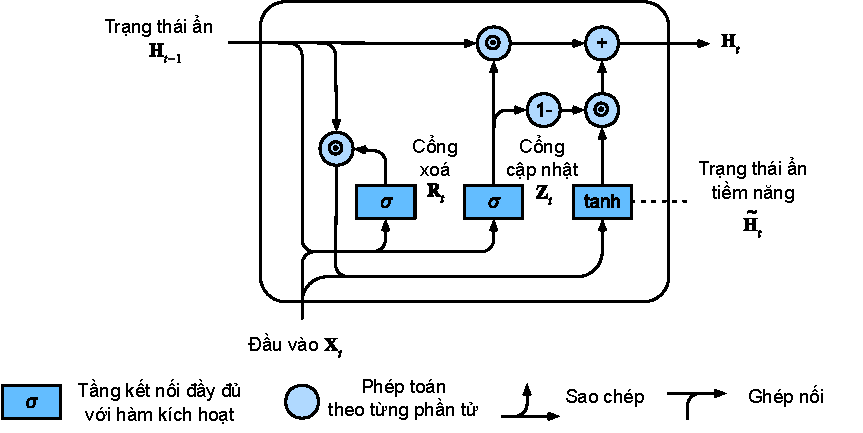
\includegraphics[width=1\textwidth]{bibliography/figure/GRU/gru_3.pdf}
        \caption{Tính toán trạng thái ẩn trong một GRU. Phép nhân được thực hiện cho từng phần tử}
        \label{fig:gru_up}
    \end{minipage}

\end{figure}

Nếu các giá trị trong cổng cập nhật $\mathbf{Z}_t$ bằng 1, chúng ta chỉ đơn giản giữ lại trạng thái cũ. Trong trường hợp này, thông tin từ $\mathbf{X}_t$ về cơ bản được bỏ qua, tương đương với việc bỏ qua bước thời gian $t$ trong chuỗi phụ thuộc. Ngược lại, nếu $\mathbf{Z}_t$ gần giá trị 0, trạng thái ẩn $\mathbf{H}_t$ sẽ gần với trạng thái ẩn tiềm năng $\tilde{\mathbf{H}}_t$. Những thiết kế trên có thể giúp chúng ta giải quyết vấn đề tiêu biến gradient trong các mạng RNN và nắm bắt tốt hơn sự phụ thuộc xa trong chuỗi thời gian. Tóm lại, các mạng GRU có hai tính chất nổi bật sau:

\begin{itemize}
    \item Cổng xoá giúp nắm bắt các phụ thuộc ngắn hạn trong chuỗi thời gian.
    \item Cổng cập nhật giúp nắm bắt các phụ thuộc dài hạn trong chuỗi thời gian.
\end{itemize}

\begin{thebibliography}{00}
    \bibitem{b1} P. T. Huong, "Linear regression, polynomial regression, and applications," Master’s thesis in science, 2015.
    \bibitem{b2} H. Choi, C. Jung, T. Kang, H. J. Kim, and I. -Y. Kwak, "Explainable time-series prediction using a residual network and gradient-based methods," in IEEE Access, vol. 10, pp. 108469-108482, 2022.
    \bibitem{b3} Doan Vo Duy Thanh, Nguyen Van Cuong, Vo Tan Phat, Le Khac Hong Phuc, Nguyen Duy Du, Nguyen Van Quang, Pham Minh Duc, Pham Hong Vinh, and Nguyen Canh Thuong. \textit{Gated Recurrent Unit (GRU)}. Accessed May 26, 2024. \url{https://d2l.aivivn.com/chapter_recurrent-modern/gru_vn.html}.
    \bibitem{b4} Nejedly P, Ivora A, Viscor I, Koscova Z, Smisek R, Jurak P, Plesinger F. Classification of ECG using ensemble of residual CNNs with or without attention mechanism. Physiol Meas. 2022 Apr 28;43(4). doi: 10.1088/1361-6579/ac647c. PMID: 35381586.
\end{thebibliography}


\end{document}
